\documentclass[a5paper,12pt,twoside]{scrartcl}

\usepackage{scrlayer-scrpage, caption, mystyle}
\usepackage[compact]{titlesec}
\titlespacing{\section}{0pt}{0ex}{0ex}
\titlespacing{\subsection}{0pt}{1ex}{0ex}
\titlespacing{\subsubsection}{0pt}{0.5ex}{0ex}
\setlength{\parskip}{0.3cm}

\graphicspath{{./Grafiken/}}

\clearpairofpagestyles{}

\setkomafont{pageheadfoot}{\sffamily\footnotesize}
\setkomafont{pagination}{}

\ohead{Seite~\pagemark}
\ihead{Tim Hilt, Emil Slomka}

\KOMAoptions{
  headsepline=true,
}

\begin{document}
\newgeometry{left=1cm, right=1cm, top=2cm, bottom=1cm}
\sffamily

{\usekomafont{disposition}\huge\centering
  Zusammenfassung --- Digitaltechnik 2\par
}

\section{Zahlendarstellung}

\begin{minipage}{.48\linewidth}
  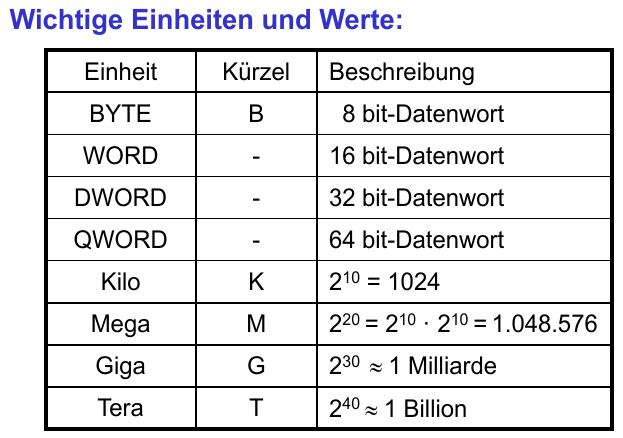
\includegraphics[width=\textwidth]{Einheiten}
\end{minipage}\hfill%
\begin{minipage}{.48\linewidth}
  \begin{center}
    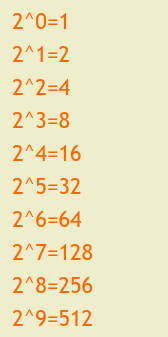
\includegraphics[width=.4\textwidth]{Zweierpotenzen}
  \end{center}
\end{minipage}

\section{KV-Diagramm}

\begin{minipage}{.43\linewidth}
  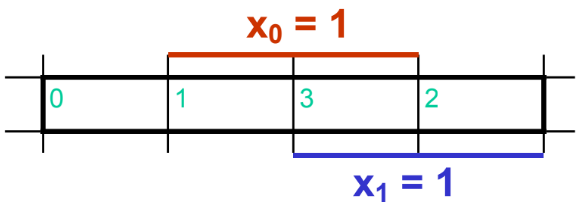
\includegraphics[width=\textwidth]{KV_Diagramm_2Eingangsvariablen}
\end{minipage}\hfill\vline\hfill%
\begin{minipage}{.53\linewidth}
  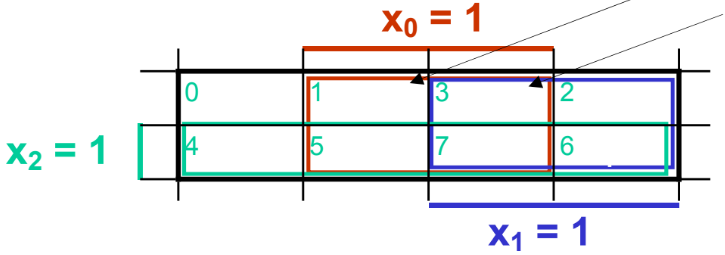
\includegraphics[width=\textwidth]{KV_Diagramm_3Eingangsvariablen}
\end{minipage}
{\centering%
  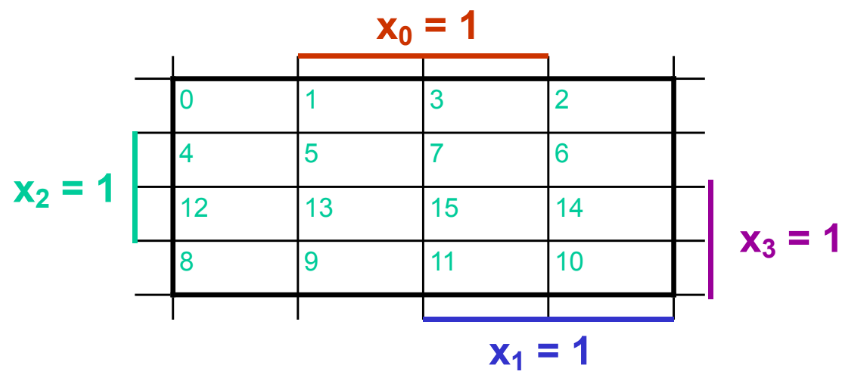
\includegraphics[width=.7\textwidth]{KV_Diagramm_4Eingangsvariablen}\par%
}

\section{Automaten}

\subsection{Automatentypen}

\begin{minipage}{.48\linewidth}
  \mybfcol{Moore-Automat}\\
  Beim Moore-Automat \textbf{hängen die Ausgangssignale nur von den Zustandsvariablen ab.} In UML erkennt man einen Moore-Automat daran, dass die \textbf{Ausgangssignale in den Zuständen} definiert sind. In einer Übergangstabelle erkennt man einen Moore Automaten daran, dass \textbf{die Ausgangsvariablen in einem Zustand für alle Kombinationen der Eingangssignale gleich} sind.
  \begin{figure}[H]
    \centering
    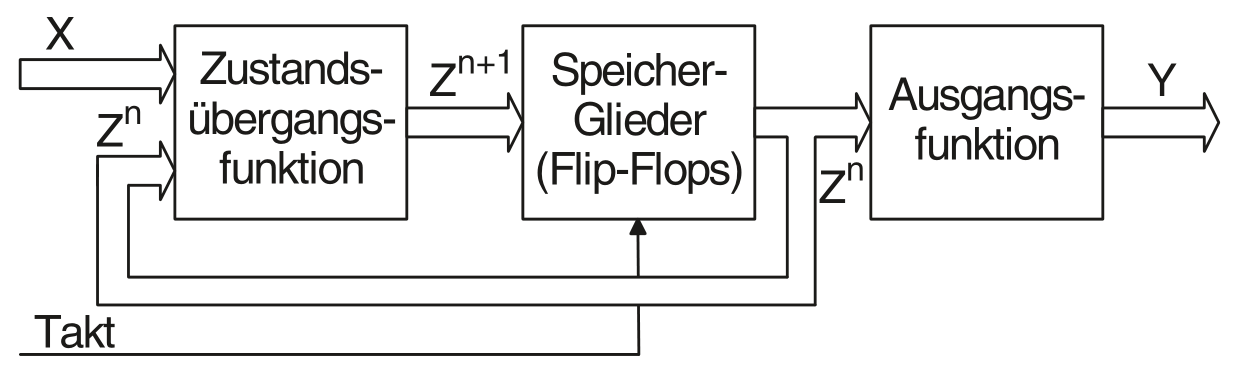
\includegraphics[width=\textwidth]{Moore_Automat}
    \caption{Moore-Automat}
  \end{figure}
\end{minipage}\hfill\vline\hfill%
\begin{minipage}{.48\linewidth}
  \mybfcol{Medwedew-Automat}\\
  Der Medwedew-Automat ist eine Sonderform des Moore-Automaten. Hier wird das Ausgangssignal nicht durch eine Ausgangsfunktion in Abhängigkeit von den Zuständen berechnet, vielmehr ist \textbf{das Ausgangssignal gleich der Zustandsvariablen.} Daher muss ein Medwedew-Automat immer gleich viele Ausgangs- wie Zustandsvariablen besitzen.
  \begin{figure}[H]
    \centering
    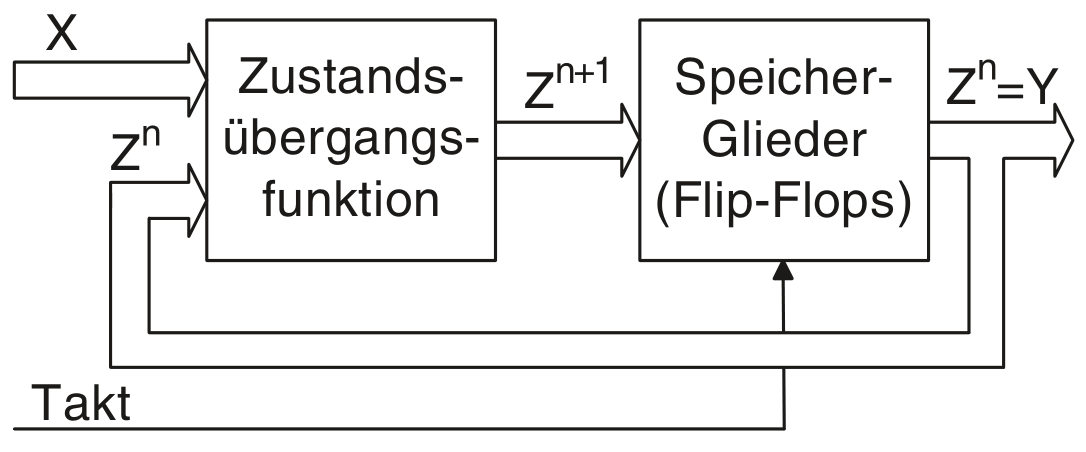
\includegraphics[width=.78\textwidth]{Medwedew_Automat}
    \caption{Medwedew-Automat}
  \end{figure}
\end{minipage}

\mybfcol{Mealy-Automat}\\
Beim Mealy-Automat \textbf{hängen die Ausgangsvariablen sowohl von den Zuständen, als auch von den Eingangsvariablen ab.} Man erkennt einen Mealy-Automaten in UML daran, dass die \textbf{Ausgangsvariablen nicht ausschließlich in den Zuständen definiert} sind. In einer Übergangstabelle erkennt man den Mealy-Automaten daran, dass das \textbf{Ausgangssignal für verschiedene Eingangskombinationen im selben Zustand unterschiedlich} sein kann.

{\centering%
  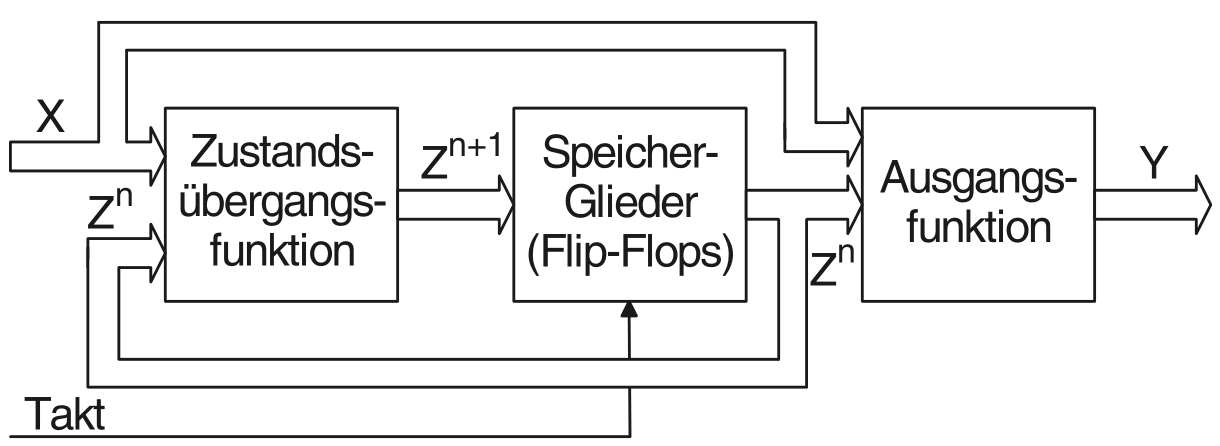
\includegraphics[width=.5\textwidth]{Mealy_Automat}
  \captionof{figure}{Mealy-Automat}\par%
}

\subsection{Realisierung eines Automaten als Zustandsdiagramm}

\begin{minipage}{.48\linewidth}
  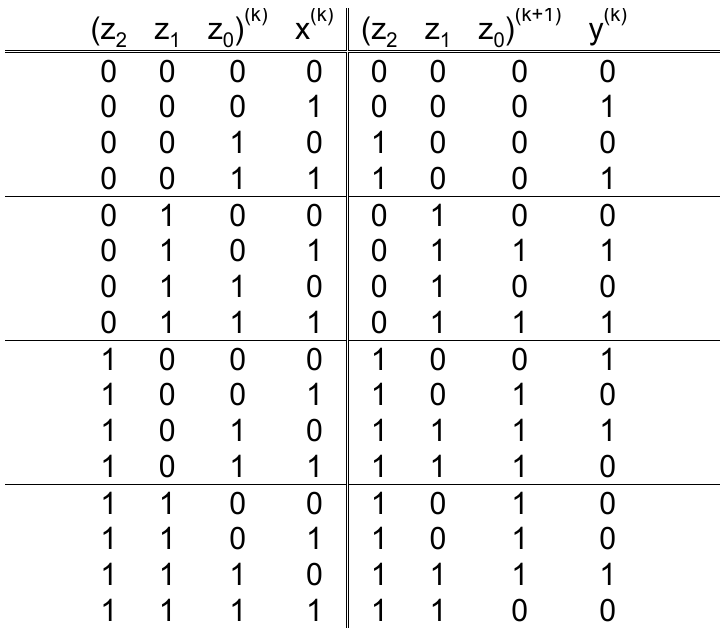
\includegraphics[width=\textwidth]{Automat_Tabelle}
  \captionof{figure}{Zustandsübergangstabelle}
\end{minipage}\hfill\vline\hfill%
\begin{minipage}{.48\linewidth}
  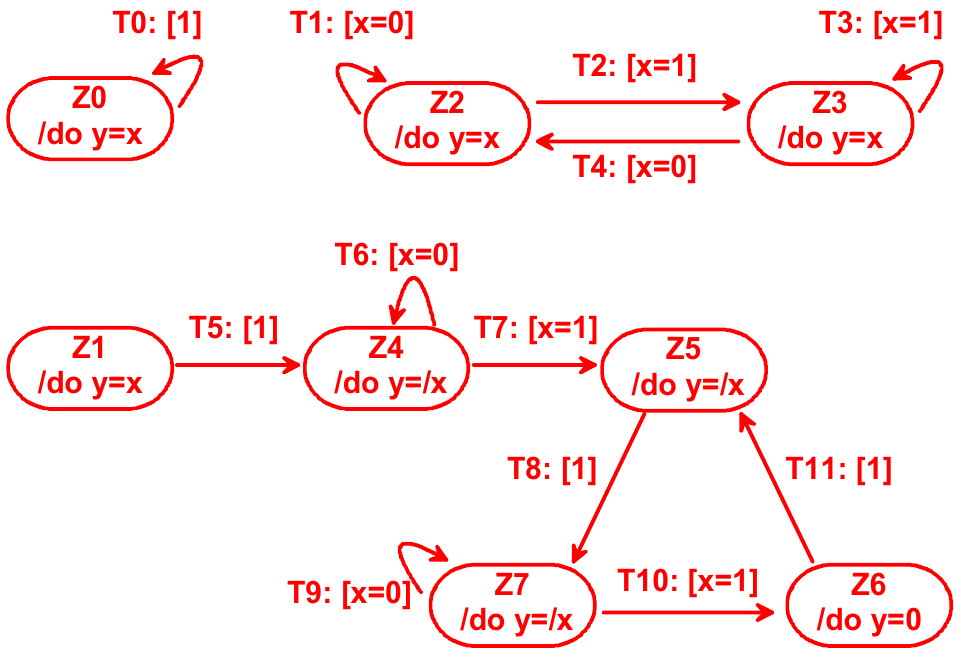
\includegraphics[width=\textwidth]{Automat_UML}
  \captionof{figure}{Zustandsdiagramm in UML-Notation}
\end{minipage}

\subsection{Realisierung eines Automaten in VHDL}

\begin{minipage}{.5\linewidth}
  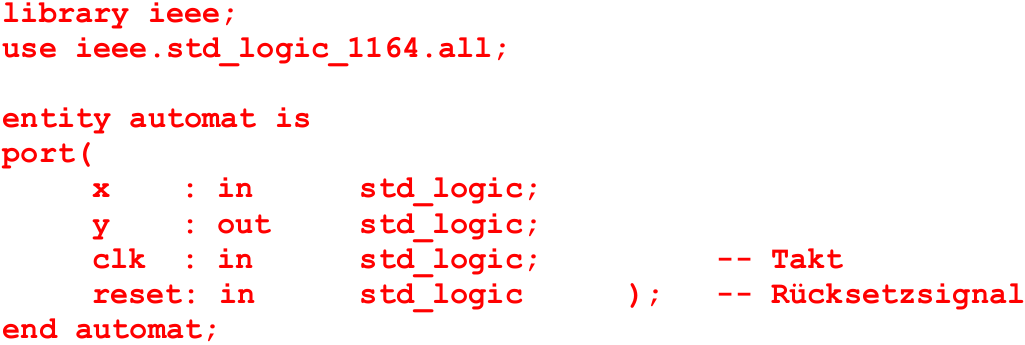
\includegraphics[width=\textwidth]{Automat_Entity}
  \captionof{figure}{Entity in VHDL}
\end{minipage}%
\begin{minipage}{.5\linewidth}
  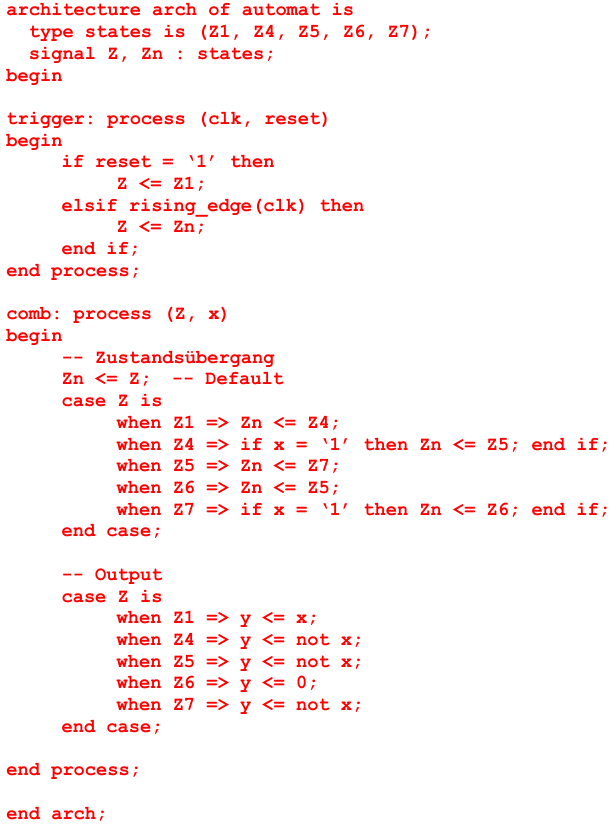
\includegraphics[width=\textwidth]{Automat_Architecture}
  \captionof{figure}{Architecture in VHDL}
\end{minipage}


\clearpage

\subsection{Realisierung eines Automaten in Hardware}

Bei gegebenem Automat in UML:\@
\begin{enumerate}
\item Stelle \textbf{Übergangs-/ Ausgangstabelle} nach folgendem Muster auf:\\[1em]
  \begin{tabular}{|cccc|cc|c|}
    \hline
    \((Z_1\) & \(Z_0)^k\) & \(x_1\) & \(x_0\) & \((Z_1\) & \(Z_0)^{k+1}\) & \(y_0\)\\
    \hline
    \hline
    \(0\) & \(0\) & \(0\) & \(0\) & \(0\) & \(1\) & \(1\)\\
    \hline
    \(\ldots\) &&&& \(\ldots\)&& \(\ldots\)
  \end{tabular}\\[1em]
  Bei \textbf{nicht spezifizierten Zuständen} werden Eingangssignale, Folgezustände und Ausgangssignale zunächst auf \textbf{don't care} gesetzt
\item Stelle \textbf{Zustandsübergangsfunktion} der Zustände \((Z_1 Z_0)^k\) zu \((Z_1 Z_0)^{k+1}\) auf; also Eingänge der Flip-Flopsauf. \mybfcol{Für \(n\) Zustände benötigt man \(n\) Flip-Flops}
  \begin{itemize}

  \item Für \textbf{D-FF}: \mytextcol{KV-Diagramm für jeweils eine Zustandsvariable des Folgezustandes} aufstellen (\(\Rightarrow Z_n^{k+1} = D_n\))
  \item Für \textbf{JK-FF}: \mytextcol{KV-Diagramm jeweils für \(J\)- und für \(K\)-Signal} aufstellen, bei \(n\) Zustandsvariablen ergeben sich \(2 \cdot n\) KV-Diagramme; jeweils \((Z)^k\) und \((Z)^{k+1}\) betrachten! Es müssen pro JK-FF zwei Spalten für \(J_n\) und \(K_n\) nach untenstehender Tabelle aufgestellt werden.
  \end{itemize}
\item Stelle \textbf{Ausgangsfunktion} auf; jeweils ein KV-Diagramm pro Ausgangsvariable; Betrachtet werden wieder die Zustandsvariablen des aktuellen Zustandes sowie die Eingangsvariablen
  \begin{itemize}
  \item \mybfcol{Notiz für Moore-Automaten:} Bei Moore-Automaten müssen bei der Berechnung der Ausgangsfunktion die \mytextcol{Eingangsvariablen nicht berücksichtigt werden}. Die Ausgangsfunktion vereinfacht sich dadurch stark
  \item \mybfcol{Notiz für Medwedew-Automaten:} Bei Medwedew-Automaten gilt \((Z_1 Z_0)^k = (y_1 y_0)\). Es müssen dabei jeweils so viele Ausgangs- wie Zustandsvariablen vorhanden sein
  \end{itemize}
\item \textbf{Zeichne Hardware als Kombination von Gattern und Flip-Flops}; Dabei werden zunächst Zustände und Eingangssignale als einzelne Leitungen geführt, die Zustände werden am Ende jedoch von den Flip-Flops rückgekoppelt und die Leitungen können gestrichen werden.
\end{enumerate}

\begin{table}[H]
  \centering
  \begin{tabular}{|cc|c|c|cc|}
    \hline
    \((Z_n)^k\) & \((Z_n)^{k+1}\)& \(D_n\) & \(T_n\) & \(J_n\) & \(K_n\)\\
    \hline \hline
    \(0\) & \(0\) & \(0\) & \(0\) & \(0\) & \(X\)\\ \hline
    \(0\) & \(1\) & \(1\) & \(1\) & \(1\) & \(X\)\\ \hline
    \(1\) & \(0\) & \(0\) & \(1\) & \(X\) & \(1\)\\ \hline
    \(1\) & \(1\) & \(1\) & \(0\) & \(X\) & \(0\)\\ \hline
  \end{tabular}
  \caption{Zustandsübergangstabelle für verschiedene Flip-Flop-Typen}
  \label{tab:FF}
\end{table}

\clearpage

\section{Speicher}

\mybfcol{Notizen zur Adressierung}
\begin{itemize}
\item Kleinste Adresse \(\Rightarrow\) Alle Bits auf 0
\item Größte Adresse \(\Rightarrow\) Alle Bits auf 1
\item Speicherbaustein auf CPU:\ Kleinste adressierbare Einheit umwandeln
\item \mytextcol{Serielle} Bausteine \(\Rightarrow\) \textbf{nacheinander} bauen
\item \mytextcol{Parallele} Bausteine \(\Rightarrow\) \textbf{nebeneinander} bauen und im Folgenden \textbf{als einen Baustein betrachten}
\end{itemize}

\mybfcol{Kleinste/Größte Adresse hexadezimal}
\begin{enumerate}
\item Speichergröße in Form \(2^{\text{Anzahl Adressleitungen}}\) schreiben
\item \(\frac{\text{Anzahl Adressleitungen}}{4}\) ergibt Anzahl von Hex-Zahlen; Rest ist Anzahl \textbf{der vorderen Bits}
\item Höchster Wert: Alle Hex-Zahlen auf \glqq{}F\grqq{} stellen, vordere Bits auf 1 setzen und als Hex-Zahl darstellen
\end{enumerate}

\textbf{Beispiel:}\\
Geg: Chip mit Speicherorganisation \(4M\):
\begin{align*}
  &= 2^{22} \rightarrow \frac{22}{4}\\
  &= 5\ R\ 2\\
  &\rightarrow \text{höchste Adresse}\ = \underbrace{11}_{\text{für Rest 2}}F.FFFF\\
  &\rightarrow 3F.FFFF
\end{align*}
\mybfcol{Merke:} Für Baustein mit Größe\\[1em]
\begin{tabular}{ll}
  \(1K\): & \(\$0400\) addieren\\
  \(2K\): & \(\$0800\) addieren\\
  \(4K\): & \(\$1000\) addieren\\
  \(8K\): & \(\$2000\) addieren\\
  \(32K\): & \(\$8000\) addieren\\
  \(64K\): & \(\$1.0000\) addieren\\
  \(256K\): & \(\$4.0000\) addieren\\
  \(512K\): & \(\$8.0000\) addieren\\
  \(1M\): & \(\$10.0000\) addieren\\
  \(2M\): & \(\$20.0000\) addieren\\
  \(16M\): & \(\$100.0000\) addieren\\
  \ldots&\\
\end{tabular}

\mybfcol{Adressraumgröße}
\[N = \underbrace{2^{(A)}}_{\text{Adressanzahl}} \times\ (\text{kleinste adressierbare Einheit})\]

\mybfcol{Anzahl Adresseingänge/Adressleitungen}
\[\log_2\left(\text{Adressanzahl}\right)\]

\mybfcol{Anzahl Bausteine parallel}
\[= \frac{\text{Datenbusbreite}\ (D)}{\text{Bitbreite Baustein}}\]

\mybfcol{Anzahl Bausteine seriell/Parallele Gruppen}
\[= \frac{\text{benötigte Anzahl Adressen}}{\text{Anzahl Adressen d. Bausteins}}\quad\text{oder:}\quad\frac{\text{benötigte Bausteingröße}}{\text{Bausteingröße}}\]



{\centering%
  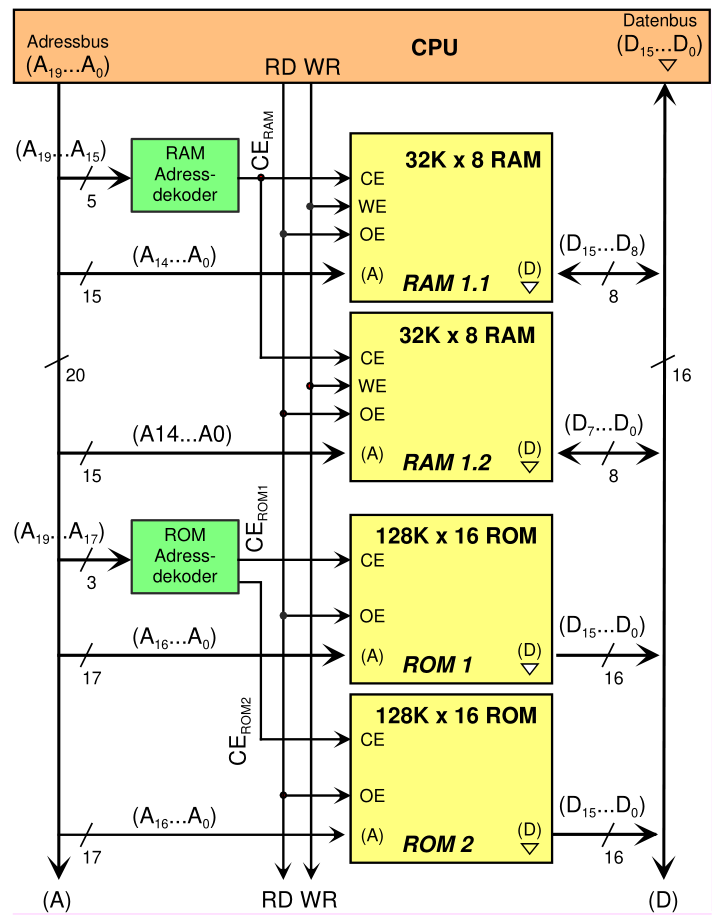
\includegraphics[width=.5\textwidth]{SpeicherAufbau}
  \captionof{figure}{Aufbau eines Speichers mit parallelen und seriellen Chips}\par%
}

\end{document}

%%% Local Variables:
%%% mode: latex
%%% TeX-master: t
%%% End:
